\section[Описание деталей реализации]{ОПИСАНИЕ ДЕТАЛЕЙ РЕАЛИЗАЦИИ}
\label{sec:realization}

Описать процесс работы программы: 
разбор консольных параметров, построение дерева Хаффмана,
выполнение побитовых операций.

Описать процесс генерации документации.

% \subsection{Установка окружения разработчика}
% \label{ssec:dev_installation}

% В этом подразделе приведено описание процесса развертывания рабочего окружения 
% для разработки сайта на Drupal: установка Apache, PHP, MySQL.
% Процесс настройки FastCGI не рассматривается, так как он является
% весьма запутанным, к тому же он достаточно подробно изложен в
% интернете, например~\cite{fast_cgi_conf}.
% В качестве базовой операционной системы выступает Debian Linux 7.0. 

% \paragraph{}
% Для создания символьного адреса сайта на локальном компьютере
% необходимо изменить файл \textit{/etc/hosts}, как показано на рисунке~\ref{lst:hosts_configuration}.

% \begin{lstlisting}[language=bash,
%   caption=Содержимое файла \textit{/etc/hosts},
%   label=lst:hosts_configuration]
% 127.0.0.1       localhost.localdomain   localhost
% ::1             localhost.localdomain   localhost

% 127.0.0.1       nagrady
% \end{lstlisting}

% Эти изменения необходимы для того, чтобы по запрос вида http://nagrady/
% в адресной строке браузера направлялся на локальный сервер, а не на удаленный.

% \paragraph{}
% Для инсталляции Drupal необходимы следующие компоненты:

% \begin{itemize}
% \item
%   веб-сервер (для приема и отправки данных);
% \item
%   база данных (для хранения данных);
% \item
%   интерпретатор PHP (для обработки данных и генерации контента).
% \end{itemize}

% В разделе~\ref{sec:choice} было установлено, что в качестве веб-сервера будет
% использоваться Apache 2.2, взаимодействующий с PHP через FastCGI,
% в качестве базы данных будет выступать MySQL 5.5.
% На данный момент последней стабильной версией PHP является PHP 5.4. 

% На рисунке~\ref{lst:web_stack_installation} приведены команды установки этих
% компонентов в ОС семейства Debian Linux.

% \pagebreak

% \begin{lstlisting}[language=bash,
%   caption=Команды установки веб-стека для работы Drupal,
%   label=lst:web_stack_installation]
% apt-get install Apache2 libApache2-mod-fcgid
% apt-get install php5 php5-curl php5-intl php5-mcrypt \ 
%         php5-mysql php5-sqlite php5-xmlrpc php5-gd php5-cgi
% apt-get install mysql-server mysql-client
% \end{lstlisting}

% В процессе установки MySQL потребуется ввести логин и пароль от учетной записи
% администратора.

% \paragraph{}
% Далее необходимо создать виртуальный хост, на котором будет размещаться сайт.
% Для этого в директории \textit{/etc/аpache2/sites-available} необходимо создать
% файл \textit{nagrady} и наполнить его содержанием, представленным на
% рисунке~\ref{lst:Apache_virtual_host}.

% \begin{lstlisting}[language=bash,xleftmargin=2em,
%   caption=Содержимое конфигурационного файла Apache,
%   label=lst:Apache_virtual_host]
% NameVirtualHost localhost
% <VirtualHost *:80>
%     ServerAdmin admin@localhost
%     ServerName nagrady
%     DocumentRoot /var/www/nagrady
%     <Directory /var/www/>
%             Options Indexes FollowSymLinks MultiViews
%             AllowOverride None
%             Order allow,deny
%             allow from all
%     </Directory>
%     ErrorLog ${APACHE_LOG_DIR}/nagrady_error.log
%     LogLevel warn
%     CustomLog ${APACHE_LOG_DIR}/nagrady_access.log combined
% </VirtualHost>
% \end{lstlisting}

% В первой строке рисунка указывается сетевое имя сервера (\textit{FQDN}). 
% Так как разработка будет производиться на том же компьютере, 
% где установлен сервер, поэтому в качестве имени выступает \textit{localhost}.
% Директива \textit{ServerAdmin} назначает почтовый адрес администратора домена, 
% \textit{ServerName} --- адрес, по которому сайт будет доступен.
% Директивы, расположенные внутри тега \textit{<Directory>}, применяются только
% к содержимому указанной директории.
% Они запрещают локальные изменения конфигурации (\textit{AllowOverride None}),
% дают доступ к файлам сайта (\textit{allow from all}),
% разрешают просматривать содержимое директорий (\textit{Options Indexes}),
% а также переходить по символическим ссылкам (\textit{Options FollowSymLinks}).
% \textit{DocumentRoot} содержит путь к файлам сайта,
% \textit{ErrorLog} и \textit{CustomLog} описывают порядок журналирования
% процесса работы сервера.

% Кроме этого, необходимо включить модули Apache, которые требуются Drupal для 
% нормального функционирования. Команды включения этих модулей и активации 
% виртуального домена приведены на рисунке~\ref{lst:Apache_configuration}.

% \begin{lstlisting}[language=bash,
%   caption=Команды включения дополнительных модулей
%   Apache и активации виртуального домена,
%   label=lst:Apache_configuration]
% a2enmod rewrite
% a2enmod fcgid
% a2dissite default
% a2ensite nagrady
% \end{lstlisting}

% \paragraph{}
% После этого необходимо произвести изменения конфигурации PHP.
% Для этого необходимо отредактировать файл \textit{/etc/php5/cgi/php.ini},
% внеся в него изменения, приведенные на рисунке~\ref{lst:php_configuration}.

% \begin{lstlisting}[language=bash,
%   caption=Измененные параметры файла php.ini,
%   label=lst:php_configuration]
% max_execution_time = 900
% max_input_time = 900
% memory_limit = 512M
% post_max_size = 64M
% upload_max_filesize = 64M
% max_file_uploads = 32M
% default_socket_timeout = 900
% \end{lstlisting}

% Параметр \textit{max\_execution\_time} устанавливает максимальное 
% время работы скрипта,
% \textit{default\_socket\_timeout} и \textit{max\_input\_time} ограничивают
% максимальное время, в течение которого может происходить ввод данных,  
% \textit{memory\_limit} устанавливает лимит на объем оперативной памяти,
% используемой интерпретатором,
% \textit{post\_max\_size} и \textit{upload\_max\_filesize} ограничивают
% максимальный объем загружаемых файлов.

% Для применения внесенных изменений необходимо перезагрузить веб-сервер. 
% Для этого нужно выполнить команды, приведенные на рисунке~\ref{lst:stack_restart}. 

% \begin{lstlisting}[language=bash,
%   caption=Команды перезагрузки веб-сервера,
%   label=lst:stack_restart]
% service php-fastcgi start
% service apache2 restart
% \end{lstlisting}

% \paragraph{}
% Для создания базы данных в СУБД MySQL достаточно выполнить команды,
% приведенные на рисунке~\ref{lst:mysql_create_db}.

% \begin{lstlisting}[language=SQL,alsolanguage=bash,
%   caption=Создание базы данных в СУБД MySQL,
%   label=lst:mysql_create_db]
% mysql -uroot -p<password>
% CREATE DATABASE nagrady;
% exit;
% \end{lstlisting}

% Значение \textit{<password>} соответствует паролю администратора СУБД.

% \paragraph{}
% После установки и настройки частей веб-стека можно
% приступить к установке Drush.

% \textit{Drush} --- консольная утилита, служащая для автоматизации действий,
% выполняемых с сайтом на Drupal~\cite{drush_about}.
% На рисунке~\ref{lst:drush_installation} приведена команда установки Drush.

% \begin{lstlisting}[language=bash,
%   caption=Команда установки Drush,
%   label=lst:drush_installation]
% apt-get install drush
% \end{lstlisting}

% После того, как были установлены и настроены Apache, MySQL, PHP и Drush,
% можно приступать к установке Drupal.

% \subsection{Установка Drupal}
% \label{ssec:drupal_installation}

% \paragraph{}
% После установки Drush установка Drupal является простой задачей.
% Достаточно перейти в директорию, где размещаются домены, обслуживаемые сервером,
% и набрать команды, приведенные на рисунке~\ref{lst:install_drupal}.

% \begin{lstlisting}[language=bash,
%   caption=Установки Drupal с помощью Drush,
%   label=lst:install_drupal]
% drush dl drupal
% mv drupal-7.28 nagrady
% \end{lstlisting}

% Таким образом мы загрузили последнюю стабильную версию Drupal в директорию,
% обслуживаемую сервером, следовательно, теперь сайт должен быть доступен через
% веб-интерфейс, как показано на рисунке~\ref{fig:drupal_install}.

% \begin{figure}[h]
%   \centering
%   {
%     \setlength{\fboxsep}{0pt}%
%     \setlength{\fboxrule}{1pt}%
%     \fbox{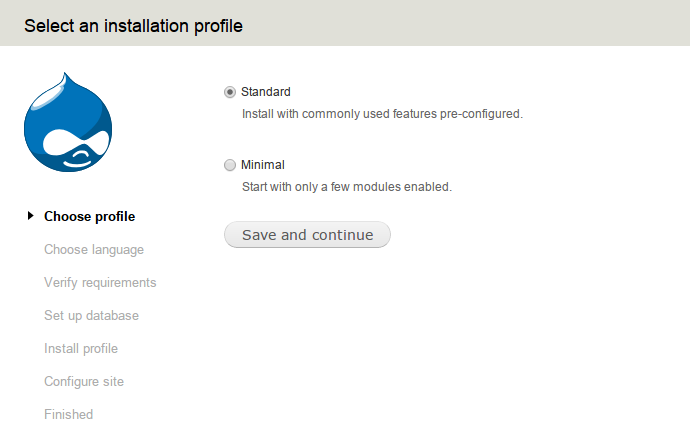
\includegraphics[width=150mm]{pic/drupal_install.png}}
%   }
%   \caption{Установка Drupal}
%   \label{fig:drupal_install}
% \end{figure}

% В ходе установки нужно будет выбрать профиль установки, 
% ввести настройки подключения к базе данных, а также логин и пароль администратора.

% После успешной установки главная страница сайта на Drupal имеет вид, 
% приведенный на рисунке~\ref{fig:drupal_after_install}.

% \begin{figure}[h]
%   \centering
%   {
%     \setlength{\fboxsep}{0pt}%
%     \setlength{\fboxrule}{1pt}%
%     \fbox{
\includegraphics[width=150mm]{pic/drupal_after_install.png}}
%   }
%   \caption{Drupal после установки}
%   \label{fig:drupal_after_install}
% \end{figure}

% \paragraph{}
% Мощность Drupal познается в его модулях. 

% \textit{Модуль Drupal} --- самостоятельная сущность, позволяющая заместить либо
% расширить стандартную функциональность ядра. 
% Модули представляют собой небольшие проекты, которые размещаются на сайте
% drupal.org и развиваются силами open-source сообщества~\cite{drupal_modules}.

% Скачать модуль можно, скачав с сайта drupal.org, и разместив в директории
% sites/all/modules сайта, либо через Drush, воспользовавшись командами,
% представленными на рисунке~\ref{lst:drush_modules}.

% \begin{lstlisting}[language=bash,
%   caption=Установка модуля Drupal с использованием Drush,
%   label=lst:drush_modules]
% drush dl <module_name>
% drush en <module_name>
% \end{lstlisting}

% В данном случае \textit{<module\_name>} соответсвует системному названию модуля,
% узнать которое можно на официальном сайте.
% Аналогичным образом устанавливаются темы оформления.

% \subsection{Обзор использованных модулей}
% \label{ssec:modules_overlook}

% В этом разделе перечисляются основные модули Drupal,
% которые были установлены и настроены с целью получения требуемой функциональности.
% Mодули сгруппированы по категориям; каждый модуль содержит краткое описание функциональности.

% \paragraph{}
% \textit{Core} --- стандартные модули Drupal. Они входят в комплект стандартной поставки Drupal.

% \textit{Block} предоставляет возможность создавать блоки. 
% Блок --- это контейнер, в котором размещается контент сайта.
% Например, список самых популярных наград на главной странице сайта является блоком.

% \textit{Contextual Links} добавляет быстрые ссылки для операций с контентом,
% видимые только администраторам.

% \textit{Image} используется для обработки изображений: изменение размера, кадрирование.
% Позволяет применять шаблоны трансформаций изображений к изображениям,
% находящимся в определенном месте сайта. Оригиналы изображений также хранятся на сайте.
% Например, оригиналы фотографии медалей имеют различные размеры. 
% Данный модуль используется для того, чтобы показывать их в заданном размере
% на главной странице, и в другом размере на странице выбранной награды.

% \textit{List} предоставляет возможность создания списков через графический интерфейс.

% \textit{Locale} предоставляет возможность локализации содержимого сайта.
% Drupal изначально имеет интерфейс на английском языке. 
% Нам требуется, чтобы наш сайт имел пользовательский интерфейс на беларуском языке.

% \textit{Menu} позволяет создавать разнообразные меню сайта из администраторского интерфейса.

% \textit{Path} позволяет изменять URL страниц сайта.

% \textit{System} обеспечивает поддержку системы конфигурирования
% для администраторов.

% \textit{Taxonomy} предоставляет возможность разделять контент по казтегориям 
% путем назначения терминов таксономии (тегов).

% \textit{Text} предоставляет возможность добавления и отображения текстовых полей.

% \textit{Update Manager} следит за обновлениями ядра и модулей,
% автоматизирует процесс обновления сайта.

% \textit{User} --- управляет системой регистрации пользователей, а также входом на сайт.

% \paragraph{}
% Группа модулей \textit{Administration Menu} добавляет удобное меню для
% пользователей с правами администратора.
% Состав пунктов меню дублирует иерархию страниц администрирования.

% \textit{Chaos Tools} предоставляет низкоуровневые функции для работы с хранением и 
% представлением контента. Требуется для установки модулей \textit{Views},
% \textit{Display Suite}, \textit{Feeds}.

% \textit{Context} используется для изменения внешнего вида отдельной страницы или 
% группы страниц в зависимости от определенного условия.
% Например, на разрабатываемом сайте этот модуль был использован для размещения блоков
% на страницах в зависимости от URL.
  
% \textit{Custom breadcrumbs} позволяет задавать содержимое breadcrumbs (<<хлебных крошек>>) 
% в зависимости от заданных условий.

% \textit{Date} предоставляет функции для работы с датой:
% ввод, валидация, хранение, представление.

% \textit{Devel} --- группа модулей, используемая для отладки.
% Предоставляет API для просмотра содержимого структур данных Drupal и его модулей,
% генерации контента, профилирования.

% \textit{Display Suite} --- группа модулей, расширяющая возможности
% \textit{Field} и \textit{Node} в области отображения контента.

% \textit{Meta Tags Quick} используется для автоматического заполнения содержимого
% SEO-тегов в зависимости от содержимого страницы.

% \textit{Administration Language} предоставляет возможность изменения языка интерфейса для
% страниц администратора.

% \textit{Localization Update} используется для автоматической загрузки обновления
% локализации интерфейса.

% \textit{Back To Top} предоставляет всплывающий виджет перемещения вверх по странице.

% \textit{Entity API} предоставляет API для работы с сущностями Drupal.
% Необходим для установки модулей \textit{Administration Views},
% \textit{views bulk operations}.

% \textit{Job Scheduler} экслпуатируется в качестве триггера другими модулями.
% Требуется для установки группы модулей \textit{Feeds}.

% \textit{Menu Item Visibility} управляет показом пунктов меню в зависимости от заданных условий.

% \textit{Module Filter} используется для фильтрации модулей по названию на соответвующей странице.

% \textit{Pathauto} автоматизирует процесс изменения URL страниц сайта.

% \textit{Token} предоставляет возможность использования переменных,
% определенных в частях Drupal, при работе с контентом.

% \textit{File Cache} используется для хранения кэша в файловой системе,
% тем самым снимая часть нагрузки с базы данных.

% \textit{Taxonomy Manager} предоставляет расширенный интерфейс для работы с таксономией.

% \textit{CKEditor} --- WYSIWYG редактор контента.

% \paragraph{}
% \textit{Feeds} --- группа модулей, предоставляющих возможность импорта данных 
% из заданного источника.

% \textit{Feeds Admin UI} --- предоставляет графический интерфейс \textit{Feeds} для администратора.

% \textit{Feeds Tamper} --- управляет отображением полей источника на поля контента Drupal. 

% \textit{Feeds Tamper Admin UI} --- предоставляет графический интерфейс
% \textit{feeds tamper} для администратора.

% \textit{Feeds Admin PHP} --- предоставляет возможность использования кода PHP для 
% для отображения данных.

% Модули этой группы используются для отображения содержимого файлов awards.csv и awarded.csv 
% на содержимое типа контента <<награжденный>> и <<награда>> соответственно. 

% \paragraph{}
% \textit{Views} --- группа модулей, ответственная за представление контента
% в разнообразной форме.

% \textit{Views Autocomplete Filters} добавляет возможность автодополнения
% к полям фильтров Views.

% \textit{Views Data Export} --- используется для экспорта данных в машиночитаемом формате.
% Например, данный модуль используется для экспорта данных о награжденных в форматах csv и xml.

% \textit{Views Dataviz} --- используется для визулизации численных данных.

% \textit{Views Date Format SQL} --- предоставляет возможность задания формата даты средствами
% языка SQL. Необходим для корректного функционирования модуля \textit{Views Dataviz}.

% \textit{Views UI} --- графический интерфейс для администрирования \textit{Views}.

% \subsection{Настройка типов контента}
% \label{ssec:content_types_setup}

% В этом подразделе рассматривается процесс настройки типов контента Drupal для хранения
% данных о награжденных и наградах.

% В соответствии с подразделом~\ref{ssub:db_info_stage}, информация о различных 
% объектах предметной области должна храниться в отдельных сущностях.
% В Drupal таким сущностям соответсвуют типы контента либо термины таксономии.

% \textit{Тип контента} представляет собой шаблон хранимых и представляемых данных и
% характеризуется определенным набором полей, задаваемых при создании.

% Всякая страница, содержащая контент, который имеент тип,
% назывется \textit{нодой} (англ. \textit{node}).

% \textit{Словарь таксономии} определяет шаблон \textit{терминов таксономии}, которые
% могут быть связаны с нодами.

% Объекту предметной области <<факт награждения>> соответствует тип контента <<узнагароджаны>>,
% представленный на рисунке~\ref{fig:awarded_content_type}.

% \begin{figure}[h]
%   \centering
%   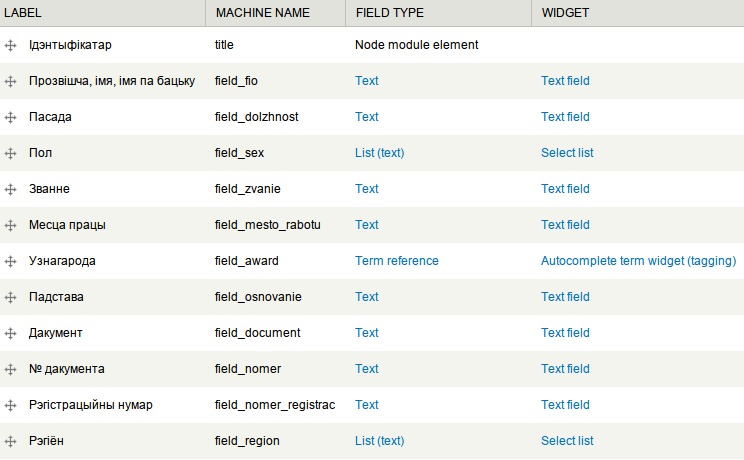
\includegraphics[width=160mm]{pic/awarded_content_type.png}
%   \caption{Тип контента <<узнагароджаны>>}
%   \label{fig:awarded_content_type}
% \end{figure}

% Объекту предметной области <<награда>> соответствует словарь таксономии <<узнагароды>>,
% представленный на рисунке~\ref{fig:awards_taxonomy}.

% \begin{figure}[h]
%   \centering
%   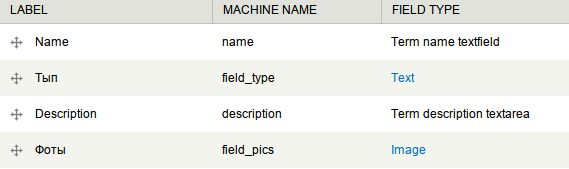
\includegraphics[width=150mm]{pic/awards_taxonomy.png}
%   \caption{Словарь таксономии <<узнагароды>>}
%   \label{fig:awards_taxonomy}
% \end{figure}

% Таким образом, термин таксономии, принадлежащий словарю <<узнагароды>>, может
% быть связан с любой нодой типа <<узнагароджаны>>.

% \subsection{Настройка импорта данных}
% \label{ssec:import_setup}

% В этом подразделе рассматриваются отображения содержимого входных файлов 
% \textit{awarded.csv} и \textit{awards.csv} на тип контента <<узнагароджаны>>
% и словарь таксономии <<узнагароды>> соответственно.

% Для импорта содержимого входных файлов в базу данных используется модули группы
% \textit{Feeds}. 

% На рисунке~\ref{fig:awards_map} приведена схема отображения данных файла
% \textit{awards.csv} на поля словаря таксономии <<узнагароды>>.

% \begin{figure}[h]
%   \centering
%   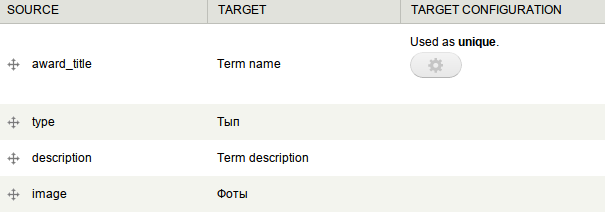
\includegraphics[width=150mm]{pic/awards_map.png}
%   \caption{Схема импорта данных о наградах}
%   \label{fig:awards_map}
% \end{figure}

% На рисунке~\ref{fig:awarded_map} приведена схема отображения данных файла
% \textit{awarded.csv} на поля типа контента <<узнагароджаны>>.
% Поле \textit{tip\_nagrady} используется в качестве ключа и состоит из полей
% \textit{fio}, \textit{nagrada}, \textit{nomer\_dokument} входного файла.

% \begin{figure}[h]
%   \centering
%   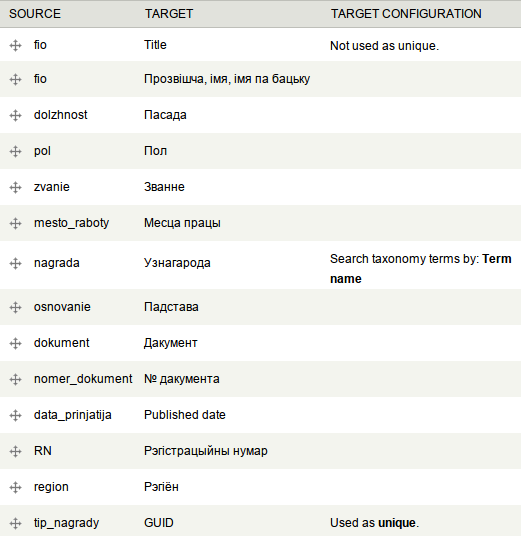
\includegraphics[width=150mm]{pic/awarded_map.png}
%   \caption{Схема импорта данных о награжденных}
%   \label{fig:awarded_map}
% \end{figure}

% Так как ноды типа <<узнагароджаны>> ссылаются на <<узнагароды>>, то
% необходимо сначала импортировать данные о наградах, а затем --- о награжденных.

% \subsection{Настройка экспорта данных}
% \label{ssec:export_setup}

% В этом подразделе рассматривается настройка экспорта данных о награжденных в 
% машиночитаемом формате.

% Для экспорта данных в машиночитаемом виде используется модули
% \textit{Views} и \textit{Views Data Export}.
% Модуль \textit{Views} используется для вывода контента, имеет множество настроек и 
% плагинов. Каждый набор настроек вывода называется \textit{видом}.

% Настройки страницы экспорта данных о награжденных приведены
% на рисунке~\ref{fig:awarded_export}.

% \begin{figure}[h]
%   \centering
%   {
%     \setlength{\fboxsep}{0pt}%
%     \setlength{\fboxrule}{1pt}%
%     \fbox{  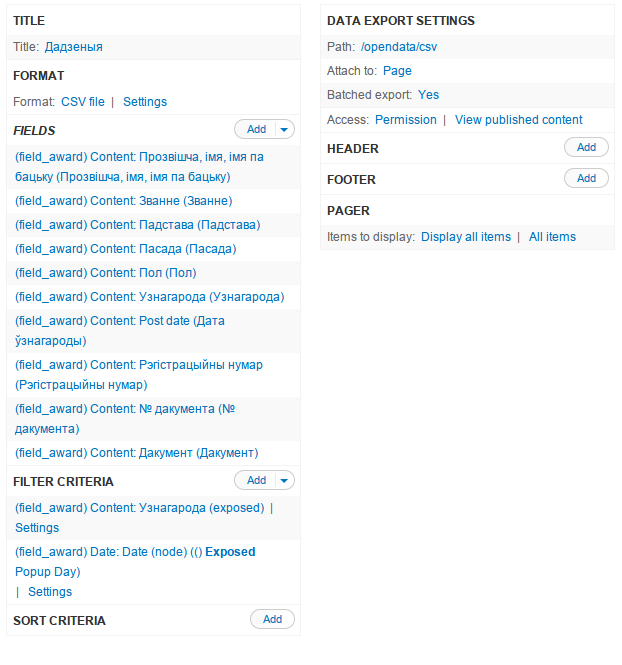
\includegraphics[width=150mm]{pic/awarded_export.png}}
%   }
%   \caption{Настройки экспорта данных о награжденных}
%   \label{fig:awarded_export}
% \end{figure}

% Данный вид позволяет пользователям производить отбор данных о награжденных
% по награде, а также по дате награждения, а также загружать данные о награжденных
% на локальный носитель.
